\chapter{Introduction} \label{sec:introduction}

The fundamental goal of the physical sciences is to understand the laws that govern physical phenomena.
This process inherently involves a continuous interplay between theoretical models and physical observations, forming a feedback loop that continuously refines both. By comparing observational data with model predictions, model validity can be tested, areas of improvements can be identified, and their faithfulness to reality can be improved. Conversely, theoretical models can guide observational strategies by predicting phenomena that have yet to be observed, hence focusing the attention to specific phenomena or conditions that may yield new insights.

A key ingredient of this scientific process is \emph{statistics}. Statistics is a rigorous mathematical language that enables formal statements about what events are possible under physical laws, thus bridging the gap between physics models and observational data. Statistics is today at the very heart of the scientific process, and not just an optional nuisance.
Guided by statistical formulation, given some parameters that describe a physical system, implied \emph{predictions} or consequences of a physical model can be computed, allowing for the systematic exploration of the model's implications. Predictions can be either deterministic or intrinsically stochastic, \eg\ due to the randomness of the physical processes, the measurement processes, or incomplete information.
In order to refine theoretical models, it is essential to perform the inverse process: starting with the effects to discover the causes, inferring from a set of observations the causal factors that produced them. This task, known as solving an \emph{inverse problem} \cite{Groetsch:1993, Aster:2005}, involves mapping back observational data to infer the underlying model parameters that are not directly observable. 

In astrophysics, this iterative cycle between prediction and inference is particularly challenging due to the complex nature of the systems under study. In this field, countless statistical methods have been developed over the years, and although rarely in the spotlight, they ultimately determine what is accepted as scientifically established truth. Since an inefficient or incorrect use of statistical data analysis may lead to weaker or entirely wrong conclusions, it is thus of the utmost importance to identify where and how progress is possible in order to advance the field. 


\section{Astrophysical data analysis challenges}\label{sec:astro}

We are at the dawn of a data-driven era in astrophysics and cosmology. As we can see from Figure~\ref{fig:intro-data}, that shows the minimum volume of data per year expected to be produced by a range of recent and upcoming surveys and experiments, the coming decade will see transformative science conducted by observatories, based both on the ground (\eg\ Rubin-LSST \cite{LSSTDarkEnergyScience:2012kar}, ELT \cite{Simon:2019aa}), and space-based missions (\eg\ JWST \citep{Gardner:2006ky}, Euclid \cite{Refregier:2010ss}). Crucially, this wealth of data promises unprecedented high-precision measurements of the growth of structure and geometry of the universe, opening new windows to dark matter \cite{Cirelli:2024ssz, drlicawagner2022reporttopicalgroupcosmic}, dark energy \cite{Mortonson:2013zfa, Huterer:2017buf}, neutrino physics \cite{Boyarsky:2012rt, SajjadAthar:2021prg}, and inflationary cosmology \cite{Baumann:2009ds, Achucarro:2022qrl}.

Given the unprecedented size and detail of these data, connecting theoretical models with this wealth of high-precision observations presents significant challenges, and the scientific return of many upcoming observations is expected to be limited by the efficiency of our statistical inference tools \cite{AlvesBatista:2021eeu, Green:2022hhj}. First, information must be optimally extracted from the data to avoid discarding valuable insights. Second, uncertainties must be correctly treated and thoroughly propagated to ensure accurate scientific statements. Moreover, fully exploiting this data for scientific purposes will require increasingly complex physical models, which bring along higher computational costs, as well as a larger number of uncertain parameters, including those characterizing signal and background systematics. Hence, the need for principled and scalable statistical analyses has never been more critical (for recent reviews on statistical analysis developments in cosmology and astrophysics see Refs.~\cite{Trotta:2017wnx, verde2010statistical, feigelson2021twenty}).

\begin{figure}
    \centering
	\includegraphics[width=\linewidth]{INTRO-data.png}
    \caption{The graphic shows rough estimates for the minimum expected volume of data per year in petabytes for a range of current and upcoming experiments and surveys in astrophysics and cosmology. Note that both the data volume and start dates are indicative; the plot is intended to give a general overview of the current and future data analysis challenges of the field. The figure and caption are a reproduction of Figure 12 in Ref.~\cite{AlvesBatista:2021eeu}.}
    \label{fig:intro-data}
\end{figure}

To get a glimpse of the types of challenges astrophysical data analysis is currently facing, we will now discuss on a high-level some exemplary problems. The selected topics cover only a small part of the current astrophysical statistical analysis challenges, and reflect the works presented in this thesis.

\paragraph{Strong gravitational lensing}
Gravitational lensing \cite{Meneghetti:2016aa}, the phenomenon where light-rays from a distant source bend due to the presence of an intervening massive object (the lens), has significantly advanced various fields of physics. Significant findings include, \eg, discovering and analysing some of the most distant galaxies in the universe \cite[\eg][]{Zitrin_2015, Naidu_2022, Treu_2015}, determining the dark matter content within galaxy clusters and understanding its distribution on both galactic and sub-galactic scales \cite[\eg][]{Dalal:2001fq, Vegetti:2014lqa, Gilman:2019nap, Hsueh:2019ynk, Nightingale:2014aa}, detecting individual light dark matter halos \cite[\eg][]{Vegetti:2009cz, Vegetti:2012mc, Hezaveh:2016ltk}, and measuring the Hubble constant \cite[\eg][]{Suyu_2020, Birrer_2020}. Crucial to many of these studies is the capability to accurately invert the physical predictive model for the source and lens. Hence, it includes dealing with very large number of degenerate parameters: for instance, variations in the source morphology (\eg, parametrized by a pixel grid, with $\mathcal{O}(\text{pixels})$ parameters \cite[\eg][]{Karchev:2021fro}), substructure population (\eg, tenth of thousands of parameters for a cold dark matter population \cite[\eg][]{Montel:2022fhv}), and main lens mass distribution. Moreover, it involves solving a mixture of parameter inference, object detection, and image reconstruction problem.
        
\paragraph{Cosmology}
Recent and upcoming large-scale structure surveys will measure galaxy distributions with unprecedented precision, improving our understanding of cosmogenesis, neutrino physics, and dark energy \cite[\eg][]{LSSTDarkEnergyScience:2012kar, EUCLID:2011zbd}. These surveys compare cosmological models to data, starting with a model of the universe's initial conditions -- an isotropic density field with small Gaussian perturbations. This field evolved through gravitational processes into today's structures, catalogued in redshift space \cite{Bond:1995yt}. By modeling early universe processes and understanding the evolution of perturbations influenced by dark matter and dark energy, large-scale structure surveys provide direct constraints on the initial density field and its evolution \cite{Jasche:2012kq}. Mapping back today's structures to constraint the initial density field requires developing advanced cosmological simulators, and accounting for non-linear transformations, mixing of spatial structure, and noise, all while exploring a multi-million-dimensional parameter space at the field level.
      
\paragraph{Point-source in sky maps} 
A striking example of how having higher-resolution data calls for more complex models that need to account for more objects, hence more parameters, hence harder inference, is given by the evolution of $\gamma$-ray observations in the galactic plane. Starting with SAS-2 satellite (1972-1073), 6 $\gamma$-ray sources and the diffuse emission were identified \cite{Sas26ps, sas2}. Two decades later, with EGRET (1991-2000), it was possible to identify up to 188 $\gamma$-ray sources, extended point sources, and resolve gas emission \cite{Casandjian:2008ky}. With Fermi-LAT \cite{Fermi-LAT:2022byn}, we have now more than 6600  $\gamma$-ray sources, highly resolved gas maps, many extended sources, the detection of the Fermi bubbles \cite{dobler2010fermi}, and an unidentified component, the so called GeV excess \cite{Goodenough:2009gk}. A physical model to describe this type of data can require, \eg, $\mathcal{O}(10^4)$ parameters for the resolved point sources alone. Moreover, some of its components have an unclear uncertainty quantification (\eg\ the gas maps). For this type of data, the statistical analysis can be thought of as a mixture of source detection and image analysis, and requires self-consistent measurement of point-source population parameters based on both detected and undetected objects.
          
The common thread behind these physical systems and their statistical challenges is that they are formally representable by large models, with the adjective ``large" describing three different properties at the same time: their complexity (in terms of number of components and potentially intricate interactions between them), their volume (in terms of observational data), and the computational resources (in terms of power, memory, and time) needed to solve them. In recent years, new classes of scalable, fast, and computational-efficient inference algorithms have been enabled by breakthroughs in machine learning \cite{Murphy:book}, which could play a major role in the successful analysis of these types of astrophysical data.


\section{The emergence of the simulation-based inference paradigm} \label{sec:paradigm}

Over the years, in order to draw scientific conclusions, an abundance of statistical tools and physics simulation codes have been developed within the community.\footnote{An extensive list of the tools used in astrophysics, cosmology, and high energy physics can be found here: \url{https://github.com/nikosarcevic/HEP-ASTRO-COSMO}.}
In particular, \emph{physics simulators} have always served as powerful predictive devices, mapping model parameters into realized data by reproducing numerically the underlying natural phenomenon of interest.
Recently, remarkable progress in computing technologies and programming languages have made it possible to express increasingly detailed and complex physical models through high-fidelity computer simulators. However, while simulators excel at predicting system behaviors, they are poorly suited for statistical inference and for solving inverse problems. 
Broadly speaking, to evaluate the likelihood of a data realization implicitly defined through a computer simulator one must solve an inverse problem that involves integrating all possible code paths, for all possible simulator configurations, that could have potentially led to the observed data realization. Clearly, as the fidelity and detail of modern computer simulations increase, computing this quantity becomes exceedingly difficult, if not entirely intractable or computationally infeasible  \cite{Cranmer:2019eaq}. 

Fortunately, recent advances in deep learning \cite{lecun2015deep} and differentiable programming \cite{baydin2018automatic} have led to the emergence and proliferation of a \emph{simulation-based inference paradigm} that can effectively tackle the above challenges. By leveraging the power of neural networks, these new methods can approximate the complex relationships within simulators, allowing for efficient solutions to inverse problems that were previously beyond reach \cite{Cranmer:2019eaq}. This paradigm shift in statistical analysis has led to the proliferation of tools for simulation-based inference \cite[\eg][]{Alsing:2019xrx, tejero-cantero2020sbi, Miller2022, lampe} and to their application to various problems in gravitational waves astronomy \cite[\eg][]{Dax:2021tsq, Crisostomi:2023tle, kolmus2024tuning, Dimitriou:2023knw, Vilchez:2024qnw, Bhardwaj:2023xph, Alvey:2023naa, Alvey:2023npw}, strong gravitational lensing analysis \cite[\eg][]{Montel:2022fhv, Wagner-Carena:2020yun, Wagner-Carena:2022mrn, wagnercarena2024strong, Coogan:2022cky, Brehmer:2019jyt, Zhang:2022djp}, cosmological probes \cite[\eg][]{List:2023aa, Tucci:2023bag, Alsing:2019xrx, Modi:2023drt, Makinen:2021nly, DES:2024xij, Jeffrey:2020aa, vonWietersheim-Kramsta:2024cks, Cole:2021gwr, FrancoAbellan:2024tbj, Saxena:2023tue, Karchev:2022xyn, Karchev:2024stw}, and many other astrophysical problems \cite[\eg][]{AnauMontel:2022ppb, Barret:2024kvc, vasist2023neural, Hahn:2022nda, khullar2022digs, Mishra-Sharma:2021oxe, Christy:2024hou, Hermans:2020skz, Alvey:2023pkx, Berteaud:2024zda, Mishra-Sharma:2021nhh}.

We will see more in depth in Chapter~\ref{cha:sbi} the technical details of the various simulation-based inference algorithms, showing how they can improve the quality of insight we can gain from simulations, maximizing information extraction from data, and providing robust uncertainty quantification for scientific statements. In the next introductory section, we will focus on providing the context and motivation for this paradigm shift, comparing it to the likelihood-based paradigm, and highlighting how it can help in tackling some of the challenges discussed previously in Section~\ref{sec:astro}.


\section{To likelihood-base or to simulation-base?}\label{sec:lbi-sbi}

Ultimately, we are interested in inferring the probability distribution of model parameters $\param$ for a given observation $\data_0$. 
%It is therefore important to begin this chapter by clearly clarifying the adopted definition of probability. Throughout this thesis, we will adopt a Bayesian view of probability. In the Bayesian paradigm, probability is a measure of plausibility and simply quantifies an observer belief about how well a quantity of interest can be measured.
In a Bayesian inference context, the posterior distribution for model parameters $\param$ follows from Bayes' theorem
\begin{equation} \label{eq:sbi-Bayes}
    p(\param\mid\data)=\cfrac{p(\data\mid\param)}{p(\data)} \, p(\param) \, ,
\end{equation}
where $p(\data\mid\param)$ is the likelihood of the data $\data$ for given parameters $\param \in \mathbb{R}^D$, $p(\param)$ is the prior probability distribution over the parameters, and $p(\data)$ is the evidence of the data.  
As evident from Equation \eqref{eq:sbi-Bayes}, the Bayesian framework needs both a formalization of the modeling assumptions, encoded by the likelihood, and a prior knowledge associated with each learnable parameter of the model, encoded by the prior. %It acknowledges that learning a model is a subjective task. Occam’s razor says we should always favour the simplest of potential explanations. The Bayesian approach may naturally handle this principle by attributing higher plausibility to simpler model instantiations.
 
Given this Bayesian setup, statistical inference is performed within the context of a probabilistic model $p(\data\mid\param)$, that can be in principle accessed by two different routes. On one hand, \gls*{lbi} algorithms rely on likelihood \underline{evaluations}, single scalars that quantify closeness to the observation $\data_0$. On the other hand, \gls*{sbi} algorithms do not explicitly calculate the likelihood function, but instead rely on \underline{samples} from a stochastic simulator that \emph{implicitly maps} model parameters $\param$ to data $\data$.

\subsubsection{Likelihood-based methods}

The main \gls*{lbi} tools to solve inverse problems for modern astrophysical and cosmological data analysis have been sampling-based inference methods, like \gls*{mcmc} \citep{Metropolis:1953am, Hastings:1970aa} and nested sampling \citep{Skilling:2006gxv, Feroz:2008xx, Ashton:2022grj} techniques. However, it is especially challenging to ensure these methods convergence in high dimensional parameter spaces (the time needed to reach convergence scales poorly with the dimensionality of the explored parameter space), for multi-modal posteriors, and curving degeneracies. More modern methods are taking up these challenges, including Gibbs samplers \cite{Smith:1993gibbs} (that rely on conditional distributions), and slice-sampling techniques \cite{Neal:aa, Handley:2015fda}. For example, the new generation nested sampler \texttt{PolyChord} \cite{Handley:2015fda}, based on slice-sampling, has at worst a $\mathcal{O}(D^3)$ scaling, whereas \texttt{Multinest} \cite{Feroz:2008xx} has an exponential scaling that emerges at high dimensions (see Figure 4 in Ref.~\cite{Handley:2015fda}).

As the dimensionality grows, sampling from the typical set of the posterior distribution becomes exponentially difficult \cite{betancourt2017conceptual}. Therefore, it is useful to resort to gradient-based algorithms, as they are able to concentrate the sampling in high posterior mass regions, despite the large number of model parameters, provided one has efficient access to accurate derivatives of the likelihood function with respect to the model parameters \cite{betancourt2017conceptual}. The most popular gradient-based method among physicist is \gls*{hmc} \cite{Duane:1987hmc, neal2012mcmc}, which is built on the formalism of Hamiltonian dynamics (as the name implies). Widely used in cosmology, it is of particular notice the application of Ref.~\cite{Jasche:2012kq}: dynamical large-scale structure inference from galaxy redshift surveys, where the parameter space is the 3D initial matter density field, of order $\mathcal{O}(10^7)$ voxels. This impressive result has been achieved with significant computational resources and by carefully tuning the so called ``mass matrix" of the \gls*{hmc}, which is not always possible. 

Lastly, it is worth mentioning \gls*{vi}, which, differently from the previously mentioned \gls*{lbi} methods, allows for the approximation of extremely high-dimensional Bayesian posteriors with simple proposal distributions by solving an optimization problem \cite{hoffman2013stochastic, zhang2018advances}. As for \gls*{hmc}, \gls*{vi}'s efficient implementation requires gradients from an end-to-end differentiable physical simulator \cite[\eg][]{caustic, Morvan_2021, sstrax}. This can be achieved with little extra effort through auto-differentiation libraries that are standard in deep learning packages \cite[\eg][]{pytorch, jax2018github}. Notably, \gls*{vi} has already been successfully applied in various astrophysical contexts \cite{regier2019cataloging, liu2023variational, Mishra-Sharma:2020kjb, Karchev:2021fro, leike2020resolving}. Of particular notice is Ref.~\cite{regier2019cataloging}, where they jointly optimize parameters for $188\times 10^6$ stars and galaxies using tera-scale datasets. We will come back to \gls*{vi} in Section~\ref{subsec:nsbi}, in order to compare it in details with its direct \gls*{sbi} counterpart. 

\subsubsection{Simulation-based methods}

Differently from \gls*{lbi} methods, \gls*{sbi} entirely relies on samples from a stochastic simulator that maps model parameters $\param$ to data $\data$. This mapping is equivalent to sampling from the model distribution $\data \sim p(\data\mid\param)$, which is effectively an implicit representation of the likelihood. As a result, in this setting one just needs a computational code that generates random samples from $p(\data\mid\param)$, that can be later used by a \gls*{sbi} algorithm. For the purpose of this thesis, a \emph{simulator/forward model} is a computer program that takes as input a vector of parameters $\param \in \mathbb{R}^D$, samples a series of internal states or latent variables, and finally produces a data vector  $\data$  as output (usually our observable). Programs that involve random samplings and are interpreted as statistical models are known as probabilistic programs, and simulators are an example \cite{Cranmer:2019eaq}. In principle, using simulators allows for the simultaneous inclusion of all relevant processes that can affect the data, regardless of whether a full probabilistic description is tractable or not, as long as they can be efficiently programmed. In this context, \emph{intractability} means one of two things: a closed-form expression of the likelihood distribution is not available, or even if available it is computationally too expensive, \eg, in the worst case, it scales exponentially with the number of parameters \cite{Leclercq:2018who, Mootoovaloo:2020ott}.

A more detailed exploration of the various \gls*{sbi} algorithms is presented in Chapter~\ref{cha:sbi}, we will now focus on the main high-level differences between \gls*{lbi} and \gls*{sbi}, drawing from the literature to highlight \gls*{sbi} advancements over \gls*{lbi} methods.


\subsubsection{Comparison: SBI vs. LBI}

\begin{figure}
	\centering
	\includegraphics[width=\linewidth]{TikZ/lbi_vs_sbi.pdf}
	\caption{\emph{Likelihood-based} inference algorithms rely on the evaluated likelihood  $L_{\data_0}(\param) $, which is a single scalar that quantifies closeness to the observation $\data_0$. \emph{Simulation-based} inference algorithms learn a function that can be evaluated on many different observations $\data_0$, determining their optimal distance measures case by case. Diagram credits: Christoph Weniger.}
	\label{fig:SBIvsLBI}
\end{figure}

The main differences between \gls*{sbi} and \gls*{lbi} methods are summarized in Figure~\ref{fig:SBIvsLBI}. In both cases, we start with a data model, $p(\data\mid\param$), which describes the probability of data $\data$ given parameters $\param$. In the \gls*{lbi} case, the strategy is a detailed analysis of the likelihood function $L_{\data_0}(\param)$, given an observation $\data_0$. To this end, simplifying, the \gls*{lbi} algorithm will suggest points $\param$ where the likelihood will be evaluated, and try to focus on regions with high density. On the other hand, \gls*{sbi} techniques do \emph{not} require a tractable (see above) likelihood-density $p(\data_0\mid\param)$ at a specific observation $\data_0$. Instead, they rely on synthetic data samples from the likelihood function $\data \sim p(\data\mid\param)$, for a range of model parameters $\param$ that are in the simplest case drawn from the parameter priors, $\param \sim p(\param)$, or in more complex cases from generative models \cite[\eg][]{Karchev:2022aa}. % Essentially, simulation-based techniques are calibrated based on samples from the \emph{generative model} or \emph{joined distribution} $\data, \param \sim p(\data\mid\param)p(\param) \equiv p(\data, \param)$.  

%While \gls*{lbi} produces results with maximal precision and usually the failure mode is over-confidence, the standard failure mode for \gls*{sbi} algorithms is under-confidence (provided correlations between $\data$ and $\param$ are fully identified).

%Classical likelihood-based inference algorithms are problem-agnostic: their performance does not directly depend on the properties, dimensionality or shape of the data $\data \sim p(\data\mid\param)$ for different model parameters $\param$; instead it \textit{only} depends on the shape of the likelihood function as a function of $\param$ for a specific piece of observation $\data_0$, $p(\data_0\mid\param)$.  This is in stark difference to simulation-based, or likelihood-free, algorithms, where the performance of a given algorithm depends critically on how (simulated and real) data $\data$ is processed, interpreted and used.  On first sight, this suggests that simulation-based algorithms are in general more difficult to use, since there are more choices to make.  However, if properly used, simulation-based techniques offer a range of advantages over likelihood-based methods, which we group here into three dimensions, which are also illustrated in 

While in principle the two frameworks converge to the same answer, when applied several practical differences emerge. We will highlight now two of the most striking disparities, but others will surface in the next chapter when the discussion becomes more technical.

\noindent \textbf{Recyclable inference.} As highlighted in Figure~\ref{fig:SBIvsLBI}, the analyzed observation $\data_0$ enters the statistical framework of \gls*{lbi} and \gls*{sbi} at different stages. In particular, \gls*{lbi} algorithms perform inference for a fixed observation $\data_0$, and must rerun from scratch for any another observation. It is thus computationally costly to perform new analysis and statistical test on the obtained results. On the other hand, we will see that \gls*{sbi} algorithms effectively learn an estimate of the probability density function that can be used to perform ``online" inference on any new data (as long as they stem from the same prior support). In this case, there is no need to rerun the whole pipeline for different observations, but just to re-evaluate the learned function on new data.\footnote{This property is not fully preserved in case of sequential \gls*{sbi} algorithms, as they prioritize achieving other types of benefits (this will be illustrated in Chapter~\ref{cha:sbi}).} Furthermore, statistical consistency tests can be performed rather quickly and efficiently. This aspect will be explored in Section~\ref{sec:test}.

\noindent \textbf{Breaking the curse of dimensionality.} When using likelihood-based techniques, in order to solve \emph{one} inference problem, like obtaining samples for marginal posterior of interest, one has to solve \emph{all} of them (joint posterior estimate). The computational overhead of generating joint samples as an intermediate step of marginal inference can be enormous, and can quickly turn an apparently easy inference task, like the measurement of a single physical parameter, into a big challenge. These cases are not uncommon, and, when possible, require problem specific care. For instance, it is common in several scenarios to analytically perform parts of the marginal integrals to reduce the parameter space in clever ways: \eg, in cosmic microwave background analysis by analytically marginalizing over power spectra amplitudes \cite{Gerbino:2019okg}, or in procedure for characterizing the contribution of unresolved point sources by integrating over their positions \cite{Mishra-Sharma:2016gis}, or in strong gravitational lensing analysis by marginalizing over the background source galaxy \cite{Vegetti:2008eg}.
% https://arxiv.org/pdf/1701.06988 point source integration in cross/auto-correlation studies

On the other hand, one key aspect of \gls*{sbi} algorithms in general is their ability to \emph{directly estimate marginal posteriors}, instead of having to first estimate the joint posterior over all parameter space, and then marginalize out nuisance parameters. A clear example of this property can be found in Ref.~\cite{Miller:2020hua}, where both \gls*{sbi} and and a nested sampler are used to sample from an ``eggbox" posterior with $D=14$ dimensions with over $10^4$ modes: the nested sample requires at least $10^7$ samples, whereas \gls*{sbi} needs three order of magnitude less samples to directly estimate the 1-dimensional and 2-dimensional marginal posteriors for the 14 parameters \cite[Figure 2 in][]{Miller:2020hua}. 

A second illustrative example of this property can be found in Ref.~\cite{Cole:2021gwr}. Analyzing cosmic microwave background data, they used \gls*{sbi} to directly estimate marginal posteriors for the six cosmological parameters of interest, while directly marginalizing over the thirteen varying nuisance parameters present in the analysis. The \gls*{sbi} analysis required only $3\times10^3$ simulations, while to obtain the same results using \gls*{mcmc} with the Planck likelihood required $5\times10^6$ simulations (since the \gls*{mcmc} must sample all the nineteen parameters). 

This, and many other comparative analysis of \gls*{sbi} and \gls*{lbi} methods, can be found in Figure~\ref{fig:sbi-lbi-lit}. The figure is meant as a very simplified comparison of \gls*{lbi} and \gls*{sbi} algorithms in the space of number of required simulations (or computational time to run the analysis) versus number of model parameters. Each work addresses different physics applications, each with its own set of challenges and variations, employing diverse types of analysis to solve them. Therefore, each reported scatter point is unique and achieves the reported scaling thanks to different properties of the various \gls*{sbi} and \gls*{lbi} algorithms employed in the specific study. The main take-away message from the plot is that, in general, \gls*{sbi} techniques are extremely scalable and simulation efficient with respect to \gls*{lbi} as a function of model parameters. One of the main reason, except for the fast evaluation time of neural networks, is their possibility to directly estimate marginal probabilities. This effectively means that we can use \gls*{sbi} algorithms to break down large problems into smaller ones, while coherently accounting for the uncertainties coming from the rest of the parameter space (as further detailed in Section~\ref{subsec:tmnre-m}). In the next chapter, we will get deeper into the technical details of \gls*{sbi} and illustrate more reasons why these techniques are promising for pushing the boundaries of the curse of dimensionality compared to likelihood-based methods (Figure~\ref{fig:sbi-lbi-cost}).

\begin{figure}
\centering
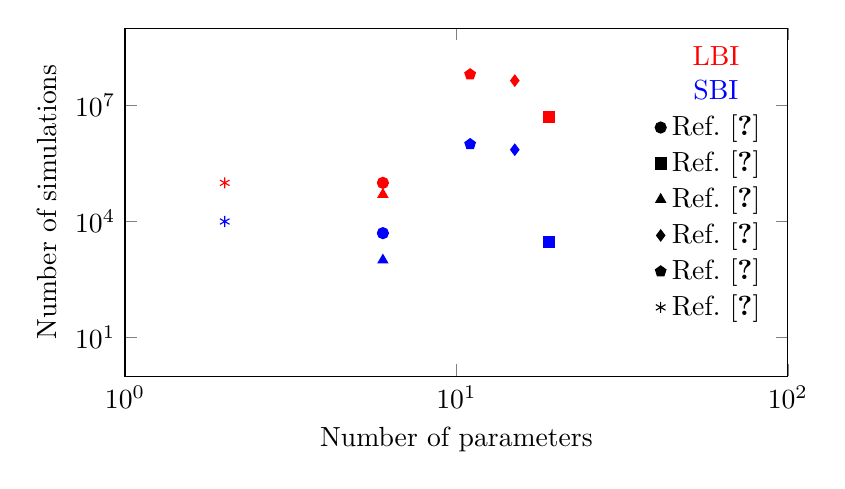
\begin{tikzpicture}
	\begin{loglogaxis}[
		width=10cm, height=6cm,
        xmin=1, xmax=1e2,
        ymin=1, ymax=1e9,
        axis line style={black},
        xlabel={{Number of parameters}},
        ylabel={{Number of simulations}},
        tick align=inside,
        minor tick style={draw=none},
        legend style={draw=none}
	]
	% Legend entries
	\addlegendimage{mark=-,red,only marks,mark size=0}
	\addlegendentry{\color{red}LBI}
	\addlegendimage{mark=-,blue,only marks,mark size=0}
	\addlegendentry{\color{blue}SBI}
	\addlegendimage{mark=*,black,only marks,mark size=2}
	\addlegendentry{Ref.~\cite{Cole:2021gwr}}
	\addlegendimage{mark=square*,black,only marks,mark size=2}
	\addlegendentry{Ref.~\cite{Cole:2021gwr}}
	\addlegendimage{mark=triangle*,black,only marks,mark size=2}
	\addlegendentry{Ref.~\cite{Alsing:2019xrx}}
	\addlegendimage{mark=diamond*,black,only marks,mark size=2}
	\addlegendentry{Ref.~\cite{Bhardwaj:2023xph}}
	\addlegendimage{mark=pentagon*,black,only marks,mark size=2}
	\addlegendentry{Ref.~\cite{Vilchez:2024qnw}}
	\addlegendimage{mark=asterisk,black,only marks,mark size=2}
	\addlegendentry{Ref.~\cite{Saxena:2023tue}}
	% Cole
	\addplot[
	    only marks,mark=*, mark size=2pt,red,
	] coordinates {(6, 1e5)};
	\addplot[
	    only marks, mark=*, mark size=2pt,blue,
	] coordinates { (6, 5e3)};
	% Cole
	\addplot[
	    only marks,mark=square*, mark size=2pt,red,
	] coordinates {(19, 5e6)};
	\addplot[
	    only marks, mark=square*, mark size=2pt,blue,
	] coordinates { (19, 3e3)};
	% Alsing
	\addplot[
	    only marks,mark=triangle*, mark size=2pt,red,
	] coordinates {(6, 5e4)};
	\addplot[
	    only marks, mark=triangle*, mark size=2pt,blue,
	] coordinates { (6, 1e3)};
	% Peregrine
	\addplot[
	    only marks,mark=diamond*, mark size=2pt,red,
	] coordinates {(15, 44e6)};
	\addplot[
	    only marks, mark=diamond*, mark size=2pt,blue,
	] coordinates { (15, 72e4)};
	% LISA gw
	\addplot[
	    only marks,mark=pentagon*, mark size=2pt,red,
	] coordinates {(11, 6.41e7)};
	\addplot[
	    only marks, mark=pentagon*, mark size=2pt,blue,
	] coordinates {(11, 1e6)};
	% 21 cm
	\addplot[
	    only marks,mark=asterisk, mark size=2pt,red,
	] coordinates {(2, 1e5)};
	\addplot[
	    only marks, mark=asterisk, mark size=2pt,blue,
	] coordinates { (2, 1e4)};
	
%	- https://arxiv.org/pdf/2403.14750 17 param (lambdacdm + nuisance)
%    - swyft 1.5 h
%    - 3 days mcmc
%- https://arxiv.org/pdf/2404.15402 kids sbi
%    - 20 min
%    - 280 min    
    
	\end{loglogaxis}
\end{tikzpicture}
\caption{Simplified comparison of likelihood-based and simulation-based algorithms in the space of number of required simulations versus number of model parameters. Each work addresses different physics applications, each with its own set of challenges and variations, employing diverse types of analysis to solve them. Therefore, each reported scatter point is unique and achieve the reported scaling thanks to different properties of the various \gls*{sbi} and \gls*{lbi} algorithms employed in the specific study.}
\label{fig:sbi-lbi-lit}
\end{figure}

\begin{figure}
    \centering
    \includegraphics[width=0.8\linewidth]{TikZ/curse_of_dim.pdf}
	\caption{Simplified comparison of likelihood-based and simulation-based algorithms in the space of number of required simulations versus number of model parameters. In general, the simulation requirements of likelihood-based techniques grows significantly with the number of model parameters (curse of dimensionality). Instead, simulation-based inference techniques can, in principle, directly focus on estimating marginal posteriors for parameters of interest, independently of the total number of parameters. This reduces the need for parameter reduction techniques and enables the comparison of complex simulation results with complex data. The figure is adapted from Figure 4 in Ref.~\cite{Boddy:2022knd}.}
    \label{fig:sbi-lbi-cost}
\end{figure}



\section{Outline}

This thesis aims to contribute to the ongoing effort to transition towards simulation-based inference techniques in astrophysics and cosmology, emphasizing some of the tremendous opportunities that this transition brings. To this end, this thesis first proposes a general simulation-based ecosystem for astrophysical data analysis (Chapter~\ref{cha:sbi}). Then, it illustrate its capabilities through exemplary applications to three challenging astrophysical problems, as motivated in Section~\ref{sec:astro}: 
\begin{itemize}[align=left, leftmargin=1cm]
	\item[{\makebox[3.2cm]{Chapters~\ref{cha:lensing} and \ref{cha:anre}: \hfill}}] The analysis of strong gravitational lenses as a dark matter {\makebox[2.45cm]{}} probe.
	\item[{\makebox[3.2cm]{Chapter~\ref{cha:cosmo}: \hfill}}] The reconstruction of cosmological initial conditions from late-{\makebox[2.45cm]{}}time density fields.
	\item[{\makebox[3.2cm]{Chapter~\ref{cha:detection}: \hfill}}] The analysis of point-sources in sky-maps. 
\end{itemize}
Overall, it aims to highlight the potential for fast, flexible, and testable simulation-based algorithms to facilitate scientific discovery in astrophysics and cosmology, at the dawn of their data-driven era, and forward.




